\documentclass[10pt, a4paper, logo, onecolumn, internal, copyright]{dsme}

\usepackage[authoryear, sort&compress, round]{natbib}
\bibliographystyle{abbrvnat}


\usepackage[utf8]{inputenc}

\usepackage{amsmath}
\usepackage{amssymb}
\usepackage{graphicx}
\usepackage{listings}
\usepackage{xcolor}
\usepackage{enumitem}
\usepackage{mdframed}

\usepackage{microtype}

\usepackage{tikz}
\usepackage{pgfplots}
\pgfplotsset{compat=1.18}

\usepackage{caption}
\usepackage{subcaption}
\captionsetup[subfigure]{justification=centering}

\usepackage{siunitx}

\DeclareCaptionType[fileext=los,placement={!ht}]{example}

\newcommand{\mpx}{\textsc{MPX}}
\newcommand{\capt}[1]{\mdseries{\emph{#1}}}

\title{\mpx{}: mixed precision Training for JAX}
\correspondingauthor{}
\reportnumber{} % Leave blank if n/a

\author[1]{Alexander Gräfe}
\author[1]{Sebastian Trimpe}

\affil[1]{RWTH Aachen University}
\date{}

\begin{abstract}
    MPX is a mixed-precision training toolbox for JAX that simplifies and accelerates the training of large-scale neural networks while preserving model accuracy. 
    MPX seamlessly integrates with popular toolboxes such as Equinox and Flax, allowing users to convert full-precision pipelines to mixed-precision versions with minimal modifications. 
    By casting both inputs and outputs to half precision, and introducing a dynamic loss-scaling mechanism, MPX alleviates issues like gradient underflow and overflow that commonly arise in half precision computations. 
    Its design inherits critical features from JAX's type-promotion behavior, ensuring that operations take place in the correct precision and allowing for selective enforcement of full precision where needed (e.g., sums, means, or softmax). 
    MPX further provides wrappers for automatic creation and management of mixed-precision gradients and optimizers, enabling straightforward integration into existing JAX training pipelines.
    \mpx{}'s source code, documentation, and usage examples are available at \url{https://github.com/AlexGraefe/mixed_precision_for_JAX}.
\end{abstract}

\begin{document}
\sloppy
\maketitle

\section{Introduction}

In recent years, JAX~\cite{deepmind2020jax} has become an increasingly popular tool for training neural networks. 
A key feature of JAX is its just-in-time compilation, which significantly accelerates code execution on hardware accelerators such as GPUs and TPUs. 
In addition, JAX supports sharding mechanisms for multi-device and multi-node training, making it easy to scale up the training of large models across entire computing clusters. 

Many libraries have been developed to extend JAX's capabilities, including Equinox, Flax, and Optax~\citep{kidger2021equinox,flax2020github,deepmind2020jax}. 
However, JAX has so far lacked a reliable, up-to-date library to enable mixed-precision training. The only existing option, JMP\citep{jmp}, is no longer maintained and cannot handle arbitrary JAX PyTrees, which are commonly used in modern neural-network toolboxes like Equinox~\citep{kidger2021equinox}.

Mixed precision training is indispensable for efficient training of large models~\cite{mixed_precision_paper}. 
By executing both the forward and backward passes of a neural network in half-precision floating-point format (requiring only \qty{16}{\bit}), mixed-precision techniques reduce memory requirements, particularly for intermediate activations, and speed up training. 
This speedup arises from lower memory transfer overhead and from specialized half-precision tensor cores in case the used hardware features them. 
Crucially, these benefits typically come without compromising accuracy.

This work presents \mpx{}, a mixed-precision training toolbox for JAX. 
\mpx{} builds on the JMP implementation and leverages Equinox's flexibility to overcome limitations in handling arbitrary PyTrees. It further introduces gradient transformations and optimizer wrappers, enabling seamless conversion of a full-precision pipeline into mixed precision with only minor modifications. \mpx{}'s source code, documentation, and usage examples are available at \url{https://github.com/AlexGraefe/mixed_precision_for_JAX}.

Before detailing the core functionality of \mpx{}, we first provide an overview of mixed-precision training. 
We then illustrate how \mpx{} can be integrated into existing workflows by presenting sample code that demonstrates its main features.

\section{Basics of mixed precision Training}
This section summarizes the original mixed precision method from NVIDIA's Automatic mixed precision \citep{mixed_precision_paper} and the paper by Micikevicius et al. \citep{mixed_precision_paper}.

mixed precision training involves performing most computations in the forward and backward passes of a neural network using 16-bit floating-point numbers. This approach offers two main advantages:
\begin{itemize}
    \item Reduced GPU memory usage (approximately 50\% compared to full precision)
    \item Potential speedup through decreased memory access times and utilization of specialized half-precision tensor cores of TPUs or GPUs.
\end{itemize}

\subsection{Loss Scaling}
A critical component of successful mixed precision training is loss scaling. Due to float16's decreased resolution, small gradients may be cast to zero, negatively impacting training performance. The solution involves:
\begin{enumerate}
    \item Scaling the loss by a factor $> 1$
    \item Calculating gradients with the scaled loss
    \item Converting gradients to float32
    \item Dividing by the scaling factor to obtain original gradients
\end{enumerate}

The scaling factor can be automatically adjusted using a simple heuristic:
\begin{itemize}
    \item If scaled gradients exceed float16 range (inf), reduce scaling and skip model update.
    \item If scaled gradients remain within float16 range for an extended period, increase scaling.
\end{itemize}

\section{Implementation Details}

\begin{figure}[t]
    \centering
    \begin{subfigure}[t]{0.99\textwidth}
        \centering
        \includegraphics[width=0.99\textwidth]{assets/EQXOverview.pdf}
        \caption{Full Precision Training via Equinox}
        \vspace{0.2cm}
    \end{subfigure}\hspace{0.1cm}
    \begin{subfigure}[t]{0.99\textwidth}
        \centering
        \includegraphics[width=0.99\textwidth]{assets/MPXOverview.pdf}
        \caption{Half Precision Training via Equinox and \mpx{}}
    \end{subfigure}\hspace{0.1cm}
    \caption{Transformation of training pipelines via MPX. \capt{An existing training pipeline (Top figure) can be transformed, by applying \texttt{@mpx.filter\_grad} to the forward pass. It automatically casts all inputs to half precision and calculates the gradient via dynamic loss scaling and \texttt{eqx.filter\_grad}.}}
    \label{fig:overview}
\end{figure}


The \mpx{} library provides essential transformations for mixed precision training while retaining JAX's low-level flexibility. 
Its design leverages JAX's type-promotion behavior\footnote{\url{https://docs.jax.dev/en/latest/jep/9407-type-promotion.html}}, ensuring that operations are performed in the precision to which the inputs and outputs have been cast—provided that all constants in the function are positioned on the left side of the type-promotion lattice. 
As such, \mpx{} primarily focuses on casting function inputs and outputs to the desired precision. 
Concretely, it first defines functions to cast PyTrees (Section~\ref{sec:castingpytrees}), then uses these to cast both functions (Section~\ref{sec:castingfunctions}) and gradient calculations (Section~\ref{sec:castinggradients}) to mixed precision. In addition, we employ dynamic loss scaling~\citep{mixed_precision_paper} (Section~\ref{sec:scaling}) to stabilize mixed precision training.

\subsection{Transformations to Cast PyTrees}
\label{sec:castingpytrees}

\mpx{} provides several functions for casting arbitrary PyTrees to a desired floating-point data type. These include
\texttt{cast\_tree(tree, dtype)}, \texttt{cast\_to\_half\_precision(x)}, \texttt{cast\_to\_float16(x)}, \texttt{cast\_to\_bfloat16(x)}, and \texttt{cast\_to\_float32(x)}. All of these functions inspect each leaf of the input PyTree, and any leaf that is a JAX array of a floating type is cast to the specified data type. Other leaves, such as integer arrays, remain unchanged.
Excluding integer arrays is important to avoid accidental casting of random generator keys.

\subsection{Transformations to Cast Functions}
\label{sec:castingfunctions}

For casting entire functions, \mpx{} provides the transformation \texttt{cast\_function(func, dtype, return\_dtype=None)}. 
This transformation returns a new function that first applies the specified input data type to all inputs (via \texttt{cast\_tree(tree, dtype)}), then calls the original function, and finally casts the outputs to the specified (optional) return data type. 
Furthermore, \mpx{} includes \texttt{force\_full\_precision(func, return\_dtype)}, which ensures computations are carried out in full precision. 
This feature is particularly important for operations that are prone to overflow in \texttt{float16}, such as \texttt{sum}, \texttt{mean}, or \texttt{softmax}.


\subsection{Automatic Loss Scaling}
\label{sec:scaling}

To facilitate the calculation of gradients via loss scaling, \mpx{} offers the class \texttt{DynamicLossScaling}, which extends \texttt{jmp.DynamicLossScaling}. This class manages dynamic loss scaling through the following methods:

\begin{itemize}
    \item \texttt{scale(x)}: Multiplies all floating-point leaves of the PyTree \texttt{x} by the current scaling factor.
    \item \texttt{unscale(x)}: Divides all floating-point leaves of \texttt{x} by the scaling factor and casts them to full precision.
    \item \texttt{adjust(grads\_finite)}: Updates the scaling factor based on the stability of the gradients, following the techniques described by \cite{nvidia_amp}.
\end{itemize}

Because \texttt{DynamicLossScaling} inherits from \texttt{eqx.Module}, it is itself a PyTree. 
Consequently, it can be used within \texttt{jit}-compiled functions and also replicated or sharded across multiple devices for distributed training.


\subsection{Transformations to Cast Gradient Calculation}
\label{sec:castinggradients}

\mpx{} provides Equinox-compatible versions of gradient-calculation functions, namely \texttt{filter\_grad(func, scaling, has\_aux=False, use\_mixed\_precision=True)} and \texttt{filter\_value\_and\_grad(func, scaling, has\_aux=False, use\_mixed\_precision=True)}. 
These functions compute gradients with mixed precision and loss scaling (as described in Section~\ref{sec:scaling}) and also automatically adjust the loss scaling value. 
They serve as drop-in replacements for the corresponding Equinox functions, allowing users to reuse existing training pipelines with minimal changes (cf. Section~\ref{sec:eqxvsmpxmodelupdate}).

To use these functions, the model's forward pass and loss computation should be combined into a single function, which is then passed to \texttt{mpx.filter\_value\_and\_grad} in place of \texttt{eqx.filter\_value\_and\_grad}. The transformed function then operates as follows (Figure~\ref{fig:overview}):

\begin{enumerate}
    \item Cast all input arguments to half precision (\texttt{float16} or \texttt{bfloat16}).
    \item Call the original function (model forward pass and loss).
    \item Scale the function's output by the current dynamic scaling factor.
    \item Apply \texttt{equinox.filter\_grad} to obtain scaled gradients.
    \item Unscale the gradients by dividing them by the scaling factor.
    \item Check whether the gradients are finite.
    \item Update the loss scaling based on the gradient's finiteness.
    \item Return a tuple containing:
    \begin{itemize}
        \item The updated \texttt{scaling} object.
        \item A boolean indicating if the gradients are finite (for the optimizer step).
        \item The computed gradients, whose format is a PyTree with the same format as the model parameters.
        \item Auxiliary values (if \texttt{has\_aux=True}).
    \end{itemize}
\end{enumerate}



\subsection{Optimizer}

Because MPX produces gradients as PyTrees, they are directly compatible with Optax optimizers~\cite{deepmind2020jax}. 
However, as discussed above, it may be necessary to skip optimizer updates altogether if the gradients become infinite due to loss scaling. 
The function \texttt{optimizer\_update(model, optimizer, optimizer\_state, grads, grads\_finite)} implements this logic and updates the model only when gradients are finite.
Consequently, instead of calling \texttt{optimizer.update} followed by \texttt{eqx.apply\_updates} (as in a typical Equinox training pipeline), one can simply call \texttt{mpx.optimizer\_update}.


\section{Example}
Here, we provide an example and show which parts in a training pipeline need to be changed for mixed precision training.

\subsection{Model Implementation}

\begin{example}[h]
    \centering
    \begin{subfigure}[t]{0.98\textwidth}
        \centering
        \begin{mdframed}[
            backgroundcolor=white!10!black,
            leftmargin=0.5cm,hidealllines=true,%
            innerleftmargin=0.2cm,innerrightmargin=0.2cm,innertopmargin=0cm,innerbottommargin=-0.10cm
        ]
            % \fontsize{8pt}{8pt}\selectfont
            \begin{lstlisting}[, escapeinside={<@}{@>},language=Python, basicstyle=\ttfamily\linespread{1.1}\footnotesize\color{white!70!black}, frame=l, label={lst:model}, keywordstyle=\color{blue!30!white}, commentstyle=\color{gray}, stringstyle=\color{orange!80!black}, numbers=left, backgroundcolor=\color{white!10!black}, numbers=left, framesep=0.8cm, framerule=0pt,  xleftmargin=0.7cm,]
grads = eqx.filter_grad(loss)(model, batch)
updates, optimizer_state = optimizer.update(
    grads, optimizer_state, eqx.filter(model, eqx.is_array))
model = eqx.apply_updates(model, updates)
            \end{lstlisting}
        \end{mdframed}
        \vspace{-0.5cm}
        \caption{Full Precision via Equinox}
        \vspace{0.5cm}
    \end{subfigure}\hspace{0.1cm}
    \begin{subfigure}[t]{0.98\textwidth}
        \centering
        \begin{mdframed}[
            backgroundcolor=white!10!black,
            leftmargin=0.5cm,hidealllines=true,%
            innerleftmargin=0.2cm,innerrightmargin=0.2cm,innertopmargin=0cm,innerbottommargin=-0.10cm
        ]
            % \fontsize{8pt}{8pt}\selectfont
            \begin{lstlisting}[, escapeinside={<@}{@>},language=Python, basicstyle=\ttfamily\linespread{1.1}\footnotesize\color{white!70!black}, frame=l, label={lst:model}, keywordstyle=\color{blue!30!white}, commentstyle=\color{gray}, stringstyle=\color{orange!80!black}, numbers=left, backgroundcolor=\color{white!10!black}, numbers=left, framesep=0.8cm, framerule=0pt,  xleftmargin=0.7cm,]
loss_scaling, grads_finite, grads = mpx.filter_grad(loss, loss_scaling)(
    model, batch)
model, optimizer_state = mpx.optimizer_update(
    model, optimizer, optimizer_state, grads,grads_finite)
            \end{lstlisting}
        \end{mdframed}
        \vspace{-0.5cm}
        \caption{mixed precision via MPX}
    \end{subfigure}
    \caption{Implementation of model updates via Equinox and \mpx{}. \mpx{} is designed such that its model update routine closely resembles the one of Equinox.}
    \label{ex:update}
\end{example}

For the largest part, the implementation of the model must not be changed. 
As \mpx{} works with arbitrary PyTrees, every Toolbox that defines their model/parameters as PyTrees, like Flax~\citep{flax2020github} or Equinox~\citep{kidger2021equinox} can be used in conjunction with \mpx{} (Listing~\ref{ex:model}). 
Only parts of the model that contain critical operations with a high risk of overflows, like sum or mean, must be transformed to full precision via \texttt{mpx.force\_full\_precision}.


\subsection{Model Updates}
\label{sec:eqxvsmpxmodelupdate}
Model updates via \mpx{} are very similar to model updates via Equinox (Figure~\ref{ex:model}). Gradients can be calulated via 


\begin{example}[h]
    \centering
    \begin{minipage}{0.95\linewidth}
    \begin{mdframed}[
    backgroundcolor=white!10!black,
    leftmargin=0.5cm,hidealllines=true,%
  innerleftmargin=0.2cm,innerrightmargin=0.2cm,innertopmargin=0cm,innerbottommargin=-0.10cm
]
        % \fontsize{8pt}{8pt}\selectfont
            \begin{lstlisting}[, escapeinside={<@}{@>},language=Python, basicstyle=\ttfamily\linespread{1.1}\footnotesize\color{white!70!black}, frame=l, label={lst:model}, keywordstyle=\color{blue!30!white}, commentstyle=\color{gray}, stringstyle=\color{orange!80!black}, numbers=left, backgroundcolor=\color{white!10!black}, numbers=left, framesep=0.8cm, framerule=0pt,  xleftmargin=0.7cm,]
class MultiHeadAttentionBlock(eqx.Module):
    dense_qs: eqx.nn.Linear
    dense_ks: eqx.nn.Linear
    dense_vs: eqx.nn.Linear
    dense_o: eqx.nn.Linear
    num_heads: int
    layer_norm: eqx.nn.LayerNorm

    def __init__(self, feature_dim, num_heads, key):
        self.num_heads = num_heads
        key, subkey = jax.random.split(key)
        self.dense_qs = eqx.nn.Linear(
            feature_dim, feature_dim, key=subkey)
        # same for dense_ks, dense_vs, dense_o

        self.layer_norm = eqx.nn.LayerNorm(feature_dim)

    def attention(q, k, v):
        attention_scores = q @ k.T / jnp.sqrt(q.shape[-1])
        <@\textcolor{white}{attention\_scores = mpx.force\_full\_precision(}@>
            <@\textcolor{white}{jax.nn.softmax, attention\_scores.dtype)(attention\_scores, axis=-1)}@>
        return attention_scores @ v
    
    def __call__(self, inputs):
        <@\textcolor{white}{inputs\_after\_layernorm = jax.vmap(mpx.force\_full\_precision(}@>
            <@\textcolor{white}{self.layer\_norm, inputs.dtype))(inputs)}@>
        qs = jax.vmap(self.dense_qs)(inputs_after_layernorm)
        qs = es.jax_einshape("n(hf)->hnf", qs, h=self.num_heads)
        # same for ks and vs...

        outputs = jax.vmap(self.attention, in_axes=(0, 0, 0))(qs, ks, vs)
        outputs = es.jax_einshape("hnf->n(hf)", outputs)
        outputs = jax.vmap(self.dense_o)(outputs)
        outputs += inputs

        return outputs
        \end{lstlisting}
        \end{mdframed}
    \end{minipage}
    \caption{Implementation of multi-headed self-attention via MPX. \capt{For the largest part, the model can be implemented in common toolboxes (here, Equinox~\cite{kidger2021equinox}). Only critical function that should be implemented in full precision, like softmax or layernorm (due to mean and std calculations), have to be transformed via \mpx{}.}}
    \label{ex:model}
\end{example}


\section{Evaluation}
We evaluate \mpx{} on two different machines: A mid-level desktop PC (AMD Ryzen 9 5950X, \qty{82}{\giga\byte} RAM, Nvidia GeForce RTX4070 GPU with \qty{12}{\giga\byte} VRAM) and a node on a high-performance cluster (CLAIX-2023, Intel Xeon 8468 Sapphire CPUs, \qty{512}{\giga\byte} RAM, four NVIDIA H100 GPUs with \qty{96}{\giga\byte} VRAM each connected via NVLink).
On paper, the desktop PC's GPU half precision computation speed is the same for half and full precision, while the H100 GPUs has double the speed for half than for full precision.

We train small vision transformers (ViT)~\cite{dosovitskiy2020image,steiner2021train}.
On both machines, the transformer has a feature size is 256, the residual blocks have one hidden layer with 800 neurons.
The desktop PC trains the ViT on Cifar100 and the high-performance cluster on ImageNet1k, equally dividing each batch between the GPUs using a data-parallel approach.
We train without gradient accumulation, which would be another way to optimize runtime and memory consumption.
We vary the number of batches and measure the time the machines need to for each training step on the entire dataset, excluding the times used for data loading.

We measure the RAM the program uses by turning off automatic preallocation and setting ``XLA\_PYTHON\_CLIENT\_PREALLOCATE'' to ``platform'', which minimizes the VRAM consumption of JAX\footnote{\url{https://docs.jax.dev/en/latest/gpu_memory_allocation.html}}
For training speed, we turn both off.

\begin{figure}[h]
    \centering
    \begin{subfigure}[t]{0.49\linewidth}
    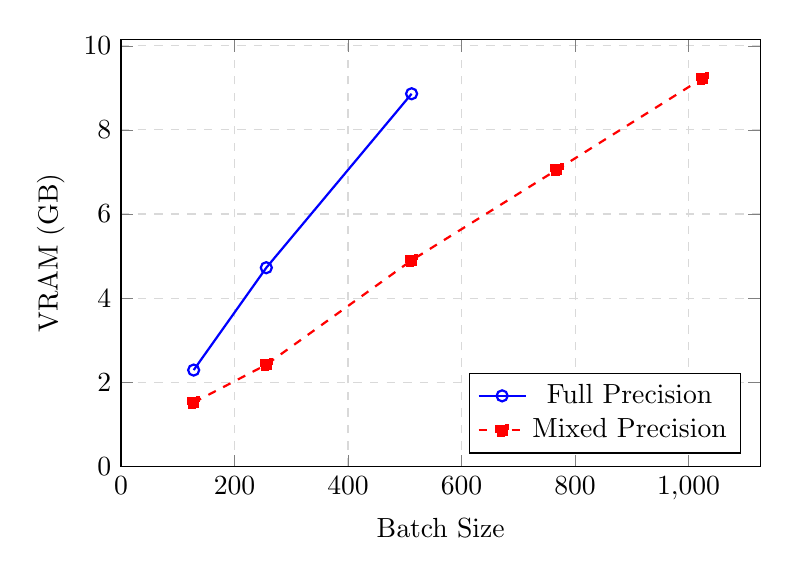
\begin{tikzpicture}
        \begin{axis}[
            width=0.8\textwidth,
            height=7cm,
            xlabel={Batch Size},
            ylabel={VRAM (\qty{}{\giga\byte})},
            legend pos=south east,
            grid=major,
            grid style={dashed,gray!30},
            xmin=0,
            ymin=0
        ]
        % First graph: Full Precision
        \addplot[
            color=blue,
            mark=o,
            thick
        ] coordinates {
            (128, 2.290)
            (256, 4.724)
            (512, 8.860)
        };
        \addlegendentry{Full Precision}

        % Second graph: Mixed Precision
        \addplot[
            color=red,
            mark=square*,
            thick,
            dashed
        ] coordinates {
            (128, 1.52)
            (256, 2.418)
            (512, 4.900)
            (768, 7.054)
            (1024, 9.222)
        };
        \addlegendentry{Mixed Precision}
        \end{axis}
    \end{tikzpicture}
    \caption{Desktop Computer (RTX4070)}
    \end{subfigure}
    \begin{subfigure}[t]{0.49\linewidth}
    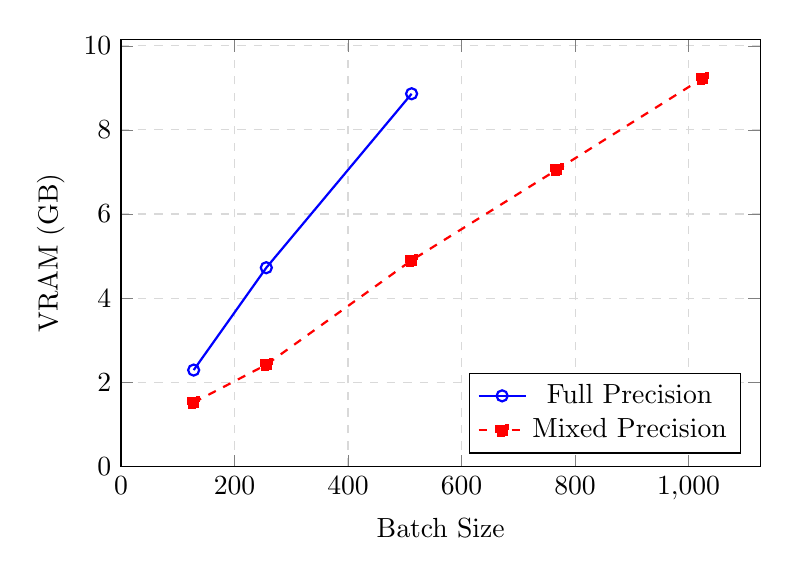
\begin{tikzpicture}
        \begin{axis}[
            width=0.8\textwidth,
            height=7cm,
            xlabel={Batch Size},
            ylabel={VRAM (\qty{}{\giga\byte})},
            legend pos=south east,
            grid=major,
            grid style={dashed,gray!30},
            xmin=0,
            ymin=0
        ]
        % First graph: Full Precision
        \addplot[
            color=blue,
            mark=o,
            thick
        ] coordinates {
            (128, 2.290)
            (256, 4.724)
            (512, 8.860)
        };
        \addlegendentry{Full Precision}

        % Second graph: Mixed Precision
        \addplot[
            color=red,
            mark=square*,
            thick,
            dashed
        ] coordinates {
            (128, 1.52)
            (256, 2.418)
            (512, 4.900)
            (768, 7.054)
            (1024, 9.222)
        };
        \addlegendentry{Mixed Precision}
        \end{axis}
    \end{tikzpicture}
    \caption{High-Performance Cluster ($4\times$ H100)}
    \end{subfigure}
    \caption{Comparison of GPU VRAM consumed for full precision and mixed precision as a function of the number of batches.}
    \label{fig:memory}
\end{figure}


\begin{figure}[h]
    \centering
    \begin{subfigure}[t]{0.49\linewidth}
    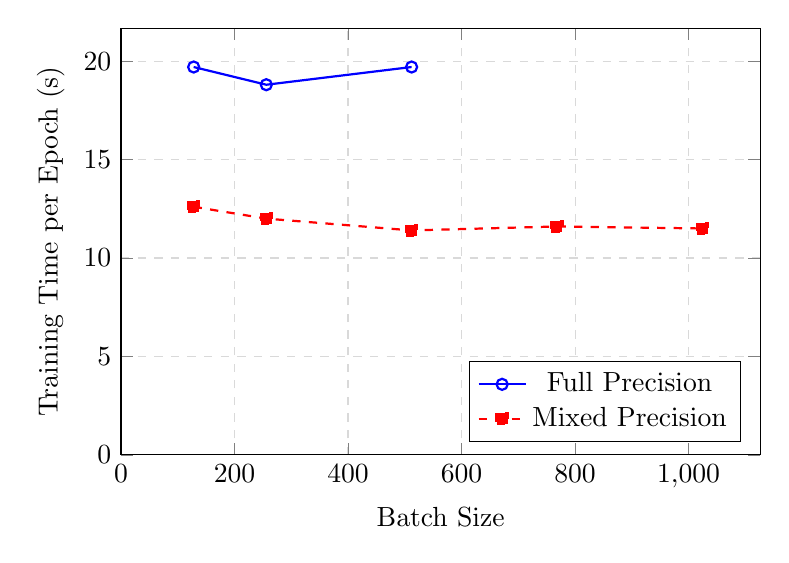
\begin{tikzpicture}
        \begin{axis}[
            width=0.8\textwidth,
            height=7cm,
            xlabel={Batch Size},
            ylabel={Training Time per Epoch (s)},
            legend pos=south east,
            grid=major,
            grid style={dashed,gray!30},
            xmin=0,
            ymin=0,
        ]
        % First graph: Full Precision
        \addplot[
            color=blue,
            mark=o,
            thick
        ] coordinates {
            (128, 19.7)
            (256, 18.8)
            (512, 19.7)
        };
        \addlegendentry{Full Precision}

        % Second graph: Mixed Precision
        \addplot[
            color=red,
            mark=square*,
            thick,
            dashed
        ] coordinates {
            (128, 12.6)
            (256, 12.0)
            (512, 11.4)
            (768, 11.6)
            (1024, 11.5)
        };
        \addlegendentry{Mixed Precision}
        \end{axis}
    \end{tikzpicture}
    \caption{Desktop Computer (RTX4070)}
    \end{subfigure}
    \begin{subfigure}[t]{0.49\linewidth}
    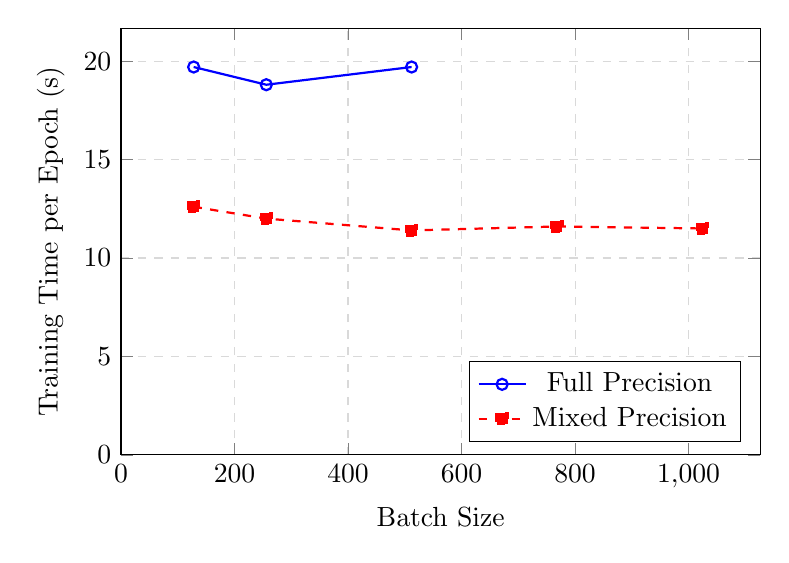
\begin{tikzpicture}
        \begin{axis}[
            width=0.8\textwidth,
            height=7cm,
            xlabel={Batch Size},
            ylabel={Training Time per Epoch (s)},
            legend pos=south east,
            grid=major,
            grid style={dashed,gray!30},
            xmin=0,
            ymin=0,
        ]
        % First graph: Full Precision
        \addplot[
            color=blue,
            mark=o,
            thick
        ] coordinates {
            (128, 19.7)
            (256, 18.8)
            (512, 19.7)
        };
        \addlegendentry{Full Precision}

        % Second graph: Mixed Precision
        \addplot[
            color=red,
            mark=square*,
            thick,
            dashed
        ] coordinates {
            (128, 12.6)
            (256, 12.0)
            (512, 11.4)
            (768, 11.6)
            (1024, 11.5)
        };
        \addlegendentry{Mixed Precision}
        \end{axis}
    \end{tikzpicture}
    \caption{High-Performance Cluster ($4\times$ H100)}
    \end{subfigure}
    \caption{Comparison of training step times for full precision and mixed precision as a function of the number of batches.}
    \label{fig:timing}
\end{figure}

Mixed precision training via \mpx{} reduces both RAM and processing times.
For the desktop PC, the RAM is reduced by factor $1.8\times$ and processing time by $1.7\times$.
The speedup is caused by reduced memory loading times as the RTX4070 features no computing speedup for half precision.

\section{Conclusion}

\mpx{} offers an easy-to-use solution for mixed-precision training in JAX.
It is able to handling arbitrary PyTrees and provides a seamless integration with popular libraries like Equinox and Flax. 
Through dynamic loss scaling and precision casting, MPX ensures efficient memory usage and accelerates training without compromising model accuracy. 
The evaluation demonstrates significant reductions in RAM usage and processing times, particularly on hardware that supports half-precision computation. 
Overall, MPX presents a compelling advancement in optimizing large-scale neural network training pipelines while maintaining flexibility and ease of use.


\section{Acknowledgements}
We express our gratitude to Patrick Kidger for Equinox and Google DeepMind for JMP, which served as the foundation for this implementation.

The authors gratefully acknowledge the computing time provided to them at the NHR Center NHR4CES at RWTH Aachen University (project number p0021919). This is funded by the Federal Ministry of Education and Research, and the state governments participating on the basis of the resolutions of the GWK for national high performance computing at universities (\url{www.nhr-verein.de/unsere-partner}).

\bibliography{references}

% \begin{thebibliography}{9}
% \bibitem{jmp} 
% JMP: JAX mixed precision
% \newblock \url{https://github.com/google-deepmind/jmp}

% \bibitem{equinox}
% Equinox: Neural Networks in JAX
% \newblock \url{https://docs.kidger.site/equinox/}

% \bibitem{nvidia_amp}
% NVIDIA Automatic mixed precision
% \newblock \url{https://developer.nvidia.com/automatic-mixed precision}

% \bibitem{mixed_precision_paper}
% P. Micikevicius et al.
% \newblock ``mixed precision Training''
% \newblock arXiv:1710.03740, 2017
% \end{thebibliography}

\end{document}
